\chapter{Introduction}

Run-time instrumentation of JavaScript (JS) is currently used for widely different
purposes.  Notable examples are automatic benchmark extraction from web
applications~\cite{Richards:2011}, empirical data gathering about the dynamic
behavior of Web applications~\cite{behavior_js} and access permission contracts
enforcement~\cite{Heidegger:2012}. All these examples require instrumentation
of object operations, such as property accesses, updates and deletion. They
also require instrumentation of all function calls made to global functions,
object methods, or function references, either directly or indirectly through
their \kw{call} or \kw{apply} method.

The standard semantics of JavaScript has no reflexion feature that completely
covers those use cases. Object-method and global-function calls can be wrapped
in closures to provide pre- and post-call instrumentation, providing a partial
solution.  However, direct calls to function references and object operations
cannot be intercepted. To work around this limitation, two main approaches are
usually employed.

In the first approach, a production virtual machine (VM), usually written in
C++, is modified to provide hooks on selected operations. It is increasingly
complex on modern JS VMs because those VMs are optimized for performance. The
resulting instrumented VM then becomes a burden to maintain up-to-date with its
evolving counterpart.

In the second approach, an \textit{ad hoc} source-to-source translator and
run-time library are written for the problem at hand and the system is expected
to run on top of a production VM. Depending on implementation choices, it can
be more or less complicated to guarantee that instrumented objects cooperate
well with the rest of the system. 

In both cases, instrumentation is achieved at a significant performance cost.
On one hand, modifications of production VMs usually are done on an interpreter
because the instrumentation hooks can break invariants assumed throughout the
JIT-compiler implementation. The modified VM will therefore at best run at
interpreter-level speed. On the other hand, source-to-source translations can
break the performance advantage of having a JIT-compiler by producing code
that is hard for the JIT-compiler to optimize.

In this dissertation, we present Photon, a framework based on \textit{virtual
machine layering}. It is inspired by previous work on metaobject
protocols~\cite{Kiczales:1991} but has been adapted to work efficiently on
modern JS VMs and provides a better separation of concerns than \textit{ad hoc}
source-to-source translations, while performing the source-to-source translation
at run time.  The optimization techniques presented in this dissertation make
Photon run 19\% faster on average  than a state-of-the-art interpreter. We
argue that it makes our approach efficient enough to replace instrumentations
that were previously targeted at interpreters on production VMs.

This dissertation therefore shows that \emph{virtual machine layering} is a
competitive alternative approach to VM instrumentation for run-time monitoring
of object operations and function calls. It makes the following contributions:
\begin{itemize}
    \item An object representation that efficiently specializes its behavior at
        run time by relying on the method caching behavior of the underlying host
        VM~(Section~\ref{sec:ObjectRepresentation});
    \item A message-sending optimization that specializes a reified operation
        to its call site by using the underlying host VM fast global function
        calls~(Section~\ref{sec:EfficientImplementation});
    \item A prototype JavaScript implementation, Photon, comprising both a runtime
        library (around 1700 lines of code) and JavaScript-to-JavaScript compiler.
\end{itemize}

\section{Overview}

In a conventional JS setting, an application runs over a high-performance host
VM. In the case of a \emph{metacircular} VM, an additional VM layer is
inserted between the application and the host VM. This layer can be a
\emph{full} or a \emph{differential} implementation. In a full implementation,
the metacircular VM provides all functionalities of the source language. In a
differential setting, however, the metacircular VM only implements parts of
the required functionality, and delegates the remaining operations to the
underlying host VM. Our approach follows a differential strategy.
Object
 operations are handled by one of the layers introduced by
Photon while primitive operations are handled by the host VM.

This section discusses the objectives that guided the design decisions,
followed by an overview of the Photon VM and its components.

\subsection{Design goals}

Our design aims to achieve the following properties:
\begin{itemize}
    \item \textbf{Isolation}: The application is isolated to avoid any
        interference with instrumentation code, while still allowing an
        instrumentation to fully inspect and modify the application state.
    \item \textbf{Flexibility}: The semantics of object operations and function
        calls are exposed as methods so that they can be extended or
        completely redefined, as required by the instrumentation.
    \item \textbf{Dynamism}: The semantics of object operations and function
        calls can be redefined while the application is running to allow
        instrumentations to precisely control the start and duration
        of their monitoring (e.g., only after the startup phase of the application).
    \item \textbf{Abstraction}: Low-level details, mostly related to
        performance optimizations, are encapsulated by specific layers to
        simplify the definition of instrumentations.
    \item \textbf{Performance}:
        Since native features provided by the host VM are often implemented
        very efficiently, our implementation reuses them when possible (e.g.,
        the scope chain and control-flow operations). Furthermore, Photon
        leverages the performance of some host feature (e.g., fast global
        function calls) to perform optimizations that reduce the overhead
        introduced by the abstraction layers.
\end{itemize}

\subsection{Overview of the Components}

\begin{figure*}[htb]
\begin{center}
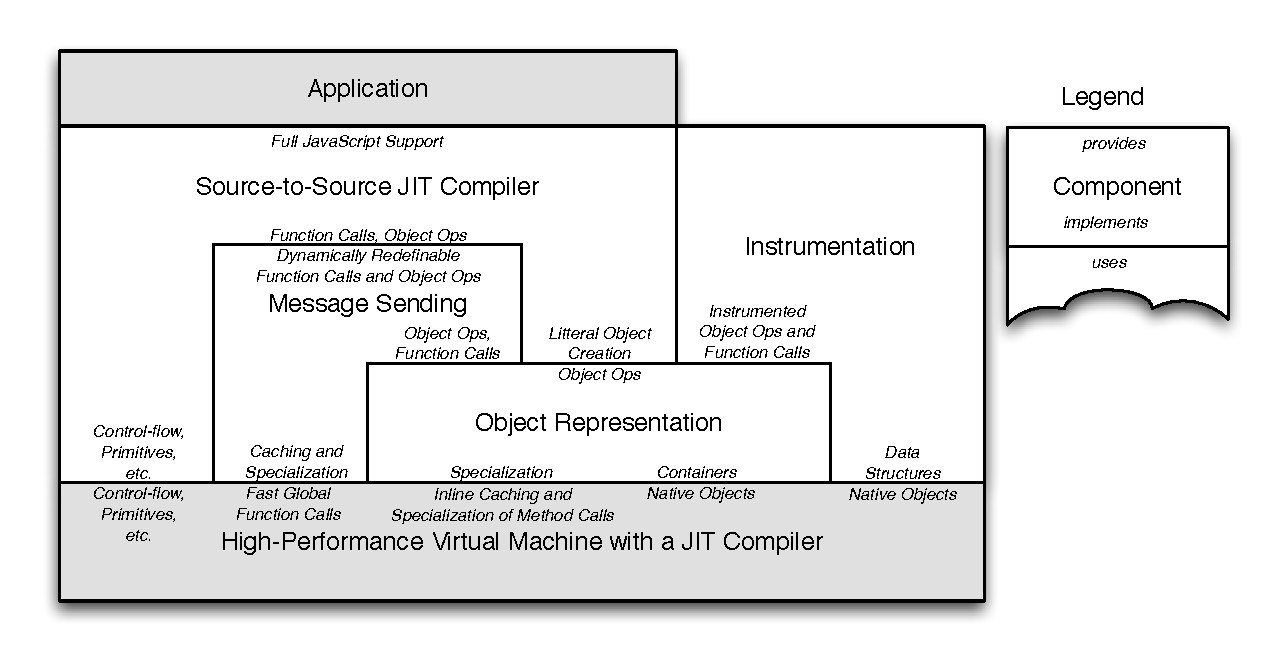
\includegraphics[width=1.0\textwidth]{figures/architecture}
\caption{\label{fig:Architecture} Components of Photon virtual machine
and the features they provide, implement and use}
\end{center}
\end{figure*}

In a conventional JS setting, we can view an application as running over a host
high-performance VM. The metacircular VM approach adds another layer between
the two, allowing instrumentations to target the middle layer instead of the
host VM.  Figure~\ref{fig:Architecture} explicits the vertical interaction
between layers by naming components and detailing which features are
implemented using features of components below it as well as the feature they
provide to the layer above. Note that the diagram represents a structural view
of component interaction and not the execution model of the application. For
example, after JIT compilation, the application code directly runs over the
host VM, albeit in a different form, although it is shown as being over the
source-to-source JIT compiler.  Note that no meaning is associated to
horizontal proximity.

We present each component, in a bottom-up fashion, in terms of the abstractions
they provide and the key features of their implementation. 

\subsection{Bottom-Up Overview}

\textbf{Object representation.} The object representation is the implementation
of JS objects (including functions) from the point of view of the Photon VM.
For efficiency, it uses native objects as property containers. The native
objects are proxied with a second native object to provide encapsulation of
invariants of the implementation in proxy methods. It has the benefit of
simplifying the implementation of instrumentations because it abstracts
implementation details required for performance. It also provides object-specific
instrumentation information to be stored on a proxy without risk of
interference with the application properties.  Object representation operations
can be specialized to certain classes of objects for performance, such as
indexed property accesses on arrays.

\textbf{Message Sending.} The message-sending layer builds on top of the object
representation to provide dynamically redefinable object operations and
function calls. This extra level of indirection is used to specialize those
operations at their call site, depending on the call site data available, such
as argument types and values, as well as the instrumentation state of the VM.
It provides dynamic optimization of uninstrumented and instrumented operations.
By implementing specialized operations as global functions, the underlying VM
will further specialize their behavior and even inline the operations in-place
when possible. The invariants implied by the implementation of the
message-sending layer are encapsulated in the object representation operations.

\textbf{Source-to-Source Compiler.} The source-to-source compiler translates
the original JavaScript code to use the run-time environment of Photon.
Non-reified elements, such as control-flow operations and primitive values and
operations are preserved.  Object operations and function calls are translated
to message sends and become dynamically redefinable. Litteral object creation
is translated to use the object representation. The source-to-source compiler
is in JavaScript and is therefore available at run-time. By staging it in front
of every call to \kw{eval}, it effectively provides a JIT compiler to Photon.

\textbf{Instrumentation.} An instrumentation can redefine the behavior
of object operations and function calls by replacing the corresponding method
on a root object with an instrumented version using the object representation
operations. The ability to completely replace a method provides maximum
flexibility to instrumentation writers compared to being limited to a specific
event before and after an operation. An instrumentation is written at the same
level as the VM, which means that it has access directly to the execution
environment of the VM and can use native objects as data structures.

\section{Background material}

To complement the introduction and overview, we elaborate on the specificities
of the JavaScript language and our definitions of object model and function
calls.

\subsection{JavaScript}

JS is a dynamic language, imperative but with a strong functional component,
and a prototype-based object system similar to that of Self.

A JS object contains a set of properties (a.k.a. fields in other OO languages),
and a link to a parent object, known as the object's prototype. Properties are
accessed with the notation \kw{obj.prop}, or equivalently \kw{obj["prop"]}.
This allows objects to be treated as dictionaries whose keys are strings, or as
one dimensional arrays (a numeric index is automatically converted to a
string).  When fetching a property that is not contained in the object, the
property is searched in the object's prototype recursively. When storing a
property that is not found in the object, the property is added to the object,
even if it exists in the object's prototype chain. Properties can also be
removed from an object using the \kw{delete} operator. JS treats global
variables, including the top-level functions, as properties of the global
object, which is a normal JS object.

Anonymous functions and nested functions are supported by JS. Function objects
are closures which capture the variables of the enclosing functions. Common
higher-order functions are predefined. For example, the \kw{map}, \kw{forEach}
and \kw{filter} functions allow processing the elements of an array of data
using closures, similarly to other functional languages. All functions accept
any number of actual parameters. The actual parameters are passed in an array,
which is accessible as the \kw{arguments} local variable. The formal parameters
in the function declaration are nothing more than aliases to the corresponding
elements at the beginning of the array. Formal parameters with no corresponding
element in the array are bound to a specific undefined value.

JS also has reflective capabilities (enumerating the properties of an object,
testing the existence of a property, etc.) and dynamic code execution
(\kw{eval} of a string of JS code).  

%Initially, our research initiative chose JS as a research object because it is
%widely used to write web applications and there is a performance gap between
%benchmarks executing on the fastest implementations of JS and compiled with
%C/C++ compilers, suggesting there are techniques to be found to close the gap.
%During exploration of VM implementation techniques, the dynamic nature of the
%language was found to be particularly well-suited to base a flexible design
%around it and initiated the work presented here. Notably, the ability to use
%the underlying JIT compiler by way of \kw{eval} and the \kw{Function}
%constructor function also enables the \textit{differential} implementation of a
%JIT compiler by adding preliminary phases to the compilation of the source
%programs.

\subsection{Object model}

An object model is a set of object kinds, their supported operations and the
time at which those operations can be performed.  Examples of object kinds are
arrays, numbers, associative arrays and classes.  Examples of operations are
object creation, addition, removal or update of properties as well as
modification of the inheritance chain. Examples of time for performing
operations are \textit{run time}, when a program is executing, \textit{compile
time}, when a program is being compiled or \textit{edit time}, when a program's
source code is being modified. An object model structures programs to obtain
properties on the resulting system such as security, extensibility or
performance. Most object models for programming languages provide an
inheritance mechanism to facilitate \textit{extensibility} by allowing an object
to be incrementally defined in terms of an existing object.

Different languages have different object models. \textit{Class-based}
object-oriented languages use \textit{class} objects to describe the properties
and the inheritance chain of \textit{instance} objects. For example, C++ class
objects exist only at compile time. Property values can be updated at run time.
Properties can only be added or removed at edit time and all their accesses are
verified at compile time. Java uses run-time objects to represent classes and
allows new classes to be added at run time.  Classes cannot be modified at run
time unless their new definition is reloaded through the debugger API. Ruby
class objects exist at run time and new properties can be added also at run
time. \textit{Prototype-based} object-oriented languages forgo the difference
between class and instance objects. Objects and their inheritance chain are
defined directly on objects. Self and JavaScript object properties can be
added or removed at run time. 

\textit{Message sending} is an operation that invokes a behavior on an object by
executing a program associated to a given message.  A message can exist at run
time and be an object like any other or it can exist only at compile time.
Message sending \textit{decouples} the intention of a program from its
implementation by adding a level of indirection between the invocation and the
execution of a given behavior. This indirection allows the behavior to change
during a program's execution. Therefore, it is a source of \textit{dynamism}.

Some languages call the program associated with a message, a \textit{method
implementation}, the message, a \textit{method name} and the act of sending a
message, \textit{method calling}. This terminology is closely tied to an
implementation strategy where the implementation is a function, the method name
is a compile-time symbol and the method call is a lookup followed by a
synchronous function call. We use the message-sending terminology because it is
more abstract. 

A message-sending object model is an object model that takes message sending as
its primitive operation. It defines every other operation in terms of message
sends. By doing so, all other operations of the object model become dynamic,
i.e. they can change at run time. By being based on a single message sending
primitive, the optimization effort can be focused on this primitive and
run-time information can be used to specialize the behavior invoked, providing
an opportunity for \textit{performance}. 

\subsection{Function-calling protocol}

The function-calling protocol is a contract between a caller and a callee
function and defines what operation each should perform before and after a
call. For implementers, it usually refers to the way arguments are
passed between the caller and the callee and who is responsible for clean-up of
shared data structures such as the stack.

In our system, there is no difference between the passing of arguments of the
host VM and the layered VM. However, to react to function-calling events, there
is a need to have a place to define operations to be executed before and after
calls. We will therefore refer to the function-calling protocol as the
operations that are performed before and after a call. 

The \kw{call} method on functions in JS is already a form of reified calling
protocol. Our design exploits it to change the behavior of \textit{all} function
calls when it is modified, which is not the case in the current standard.

%\section{VM paradigm vs instrumentation}
%
%It can legitimately be asked what the difference is between a metacircular VM
%executing on top of an existing VM and a system that would perform
%source-to-source translation at run time. This difference is mostly conceptual
%and users of these systems need not know the difference. However, there seems
%to be a fundamental difference that governs the range of implementation
%techniques available to the implementer: what assumption is made about the
%possibility of source code inadvertently interfering with implementation code.
%In other words, does the system make an \textit{open-world} assumption or a
%\textit{closed-world} assumption.
%
%In the first case, we will say that the system performs instrumentation of the
%source code. In the second case, we will say that the system can be considered
%a virtual machine, running on top of another virtual machine. 
%
%Our system makes a closed-world assumption to use the JavaScript global object
%for optimizations of implementation mechanisms.

\section{Outline}

The remainder of this dissertation covers the following subjects: 
\begin{itemize}
    \item Chapter~\ref{chap:PreviousWork} presents previous work on flexible computer systems.
    \item Chapter~\ref{chap:Design} explains the design of the VM with a
        particular emphasis on the message-sending foundation and the object
        representation.
    \item Chapter~\ref{chap:Flexibility} presents use cases in modifying the VM
        that are either difficult or impossible to do with existing JS
        implementations.
    \item Chapter~\ref{chap:Performance} compares our implementation with a
        state-of-the-art implementation to establish the overhead of providing
        the flexibility and show suitability to replace existing instrumented
        interpreters.
    \item Finally, the conclusion in Chapter~\ref{chap:Conclusion} explains the
        current limitations of the system and sketches ideas for further work
        using our current results
\end{itemize}
